\documentclass[a4paper,12pt]{article}

\usepackage[in]{fullpage}
\usepackage{parskip}
\usepackage{tikz}
\usepackage[backend=bibtex,style=numeric-comp,sorting=nyt,sortcites=true]{biblatex}
\usepackage[section]{placeins}

\title{Qualifying Dissertation}
\author{James Baxter}
\date{}

\bibliography{literature} 

\newcommand{\Circus}{{\sffamily \slshape Circus}}

\begin{document}
\maketitle

\section{Introduction}

% need a short paragraph describing the structure of the Introduction

\subsection{Motivation}

Since its release in 1995, the Java programming language~\cite{gosling2013} has
increased in popularity and is now used on a wide variety of platforms.  This
popularity means that Java has been used in a wide variety of areas including
desktop applications, on the internet in the form of Java applets, on
smartcards~\cite{chen2000} and on mobile devices~\cite{oracle2014}.  Several
languages derived from Java have also been created, including
Scala~\cite{lausanne2015} and Ceylon~\cite{redhat2015}, as well as older
variants of Java such as MultiJava~\cite{clifton2006} and
Pizza~\cite{odersky1997}, which have in turn contributed to the development of
Java. Scala adds functional programming features to Java, some of which have
been incorporated into Java 8. Ceylon extends Java's type system with features
such as union types, correcting some common Java errors in the process.
% add a short sentence describing each langauage, try to find more non-webpage references

One use of Java that is of particular interest is its use in embedded systems.
While early versions of Java were developed with the intention of using them on
embedded systems, particularly TV set-top boxes, the technology was not well
received and it was only in the growing sector of the internet that Java
intitially found a market. % need citation for this - horstmann2002?
However, it was soon realised that the portability, modularity, safety and
security benefits of Java could be of great use in embedded
systems. % need citation for this
This required the creation of specialised Java virtual machines as the standard
JVM is too large for most embedded systems and much research has gone into
making increasingly smaller virtual machines to increase the range of devices
that Java can be used on~\cite{caska2011,thomm2010}.

Many embedded systems are also real-time systems, but features of Java such as
the garbage collector and the concurrency model make it unsuitable for real-time
systems, where strict guarantees about timing properties must be made.  To
rectify these problems the Real-Time Specification for Java
(RTSJ)~\cite{gosling2000} was created.  The RTSJ extends Java with a scoped
memory model and a more predictable scheduling system, which allow RTSJ programs
to fulfil real-time requirements.

While the RTSJ addresses real-time requirements of embedded systems, many
embedded systems are also safety-critical.  Safety-critical programs must
usually be shown to conform to certain standards of safety such as,
\mbox{DO-178C} and ISO~26262, and so must be amenable to static analysis in
order to determine if they meet the required standards.  To support the
development of safety-critical programs that meet these requirements in Java,
the Safety-Critical Java (SCJ) specification~\cite{locke2013} has been created.
SCJ is a subset of the RTSJ that contains only the features that can be
statically reasoned about, which means that features such as the
garbage-collected heap and dynamic class loading are absent from SCJ.  This
facilitates the creation of SCJ programs that fulfil formal specifications;
indeed work has already been done on developing correct SCJ programs from formal
specifications~\cite{cavalcanti2011, cavalcanti2013}.

While it can be shown that SCJ programs are correct, it must still be ensured
those programs will be run correctly.  In the case of Java this generally means
ensuring the Java compiler and Java Virtual Machine (JVM) are correct. 

Work has been done in the the past on modelling virtual machines for Java, and
on the formal correctness of compilers targetting those virtual machines.  Some
of the most complete work in that area was by St\"{a}rk, Schmid and
B\"{o}rger~\cite{stark2001}, who present a model of the full Java language and
virtual machine, along with a formally verified compiler, although for an older
version of Java than is current.  Other work has also been done on modelling the
JVM and Java compilation using refinement
techniques~\cite{duran2010}. Additionally there has been work considering
machine checked models of Java virtual machines and
compilers~\cite{lochbihler2012, nipkow2000, strecker2002}. Work has also been
done apart from consideration of Java compliers on the semantics of Java
bytecode and verification of standard JVMs~\cite{bertelsen2000, jones1998}.

However, SCJ has a number of differences from standard Java. Firstly, the SCJ
memory model is rather different to the standard Java memory model, abandoning
the garbage collector in favour of a scoped memory model.  Garbage collection is
less predictable and often quite complex, and so difficult to reason about and
unsuitable for some of the strictest certifiability requirements of
safety-critical systems.  By contrast, the scoped memory model provides greater
predictability on when memory is freed as it can be determined when a particular
scope has been left.  Similarly, the SCJ approach to scheduling differs from
that of standard Java, using a preemptive priority scheduling approach rather
than the unpredictable scheduling of standard Java threads.  These differences
of SCJ from standard Java mean that the standard JVM is not suitable for running
SCJ programs.  A specialised virtual machine is required and the specialised
virtual machine must also be verified.

In the case of virtual machines for embedded systems, the priorities are usually size and
speed, which generally results in machines that are hard to verify.  In any
case, virtual machines that rely on interpreting bytecode are unsuitable for
real-time embedded systems as they are likely to be slower than running native
code directly.

An alternative method to run a Java program is to compile it to native code and
some authors have suggested doing so either directly~\cite{schultz2003} or via
C~\cite{varma2004}. There are also several virtual machines that take this
approach including Fiji VM~\cite{pizlo2009}, Icecap HVM~\cite{sondergaard2012}
and OVM~\cite{armbruster2007}.  This allows correct running of an otherwise
correct SCJ program to be viewed as a compiler verification problem.

There has been much research in the past into compiler correctness as correct 
compilation is important to the correct functioning of a program, even when the
program itself has been shown to be correct.  Much of the work follows a
commuting diagram approach, in which the compilation is shown to be consistent
with transformation between the semantics of the source and target
languages\cite{morris1973, thatcher1979}. This approach is apparent in much of the early work such as that of McCarthy and Painter~\cite{mccarthy1967}, as well as in more recent work such as the CompCert project~\cite{leroy2009a, leroy2009b}. There has also been work done using this approach in automated theorem provers~\cite{klein2006, milner1972, nipkow2000}, which provide additional certainty that the proof is correct and can also provide code generation facilities to allow creation of a working compiler.

An alternative approach to compiler verification is the algebraic approach~\cite{hoare1991, sampaio1993}, based on modelling compilation using refinement calculus~\cite{back1981, morgan1990, morris1987}. This approach appears to be less commonly used but has been applied to Java~\cite{duran2005, duran2010} and hardware description languages~\cite{perna2010, perna2011}. This approach is also quite amenable to automation as it relies on refinement laws that can be applied by a term rewriting system.

There is a clear need for formal verification of SCJ virtual machines due to the safety-critical nature of the systems involved and the fact that safety standards such as DO-178C require it at the highest safety levels. However, there appears to be little work done in that area and no known SCJ virtual machines have been formally verified.

% explain that there is a gap with no verification for SCJ compilers for embedded systems

\subsection{Objectives}

Given that there is a need for a formally verified virtual machine that can run SCJ programs efficiently on an embedded system, my objective is to identify the requirements of such a virtual machine. These requirements will be expressed in formal notation so as to permit proofs of correctness, and allow verification and construction of provably correct virtual machines.

As many existing SCJ virtual machines, particularly those targetting embedded systems, take the approach of compiling Java bytecode to native code in order to improve speed, formal specification of a SCJ virtual also includes the specification and verification of such a compiler. This must be done in addition to ensuring the virtual machine caters for the requirements of SCJ with regard to areas such as scheduling and memory management.

\subsection{Document Structure}

% Description of SCJ and review of SCJ VMs - use stuff from JTRES paper, maybe extend it a bit
% Review the literature on compiler correctness 
%  - Two approaches: algebraic and commuting diagram
%  - Consider each approach in a separate subsection and compare them
%  - Make sure to descibe the *approach* in detail, not what the authors did
%  - Finish by looking at and comparing some of the work on Java compilation
% Present research proposal and preliminary results
% - Overall plan - requirements for an SCJVM - explain different parts of the diagram, mention CEE will be dealt with by later work
% - Present the identification of the requirements for the VM services from the JTRES paper
% - Discuss the formal model - similar to JTRES paper but room to go into more depth

\section{Literature Review}

As the correctness of the compiler is of great importance to the correctness of the programs produced using it, there has been much research in the past into compiler correctness.
The approach that was used in the earliest works on compiler correctness, which is still widely used today, is to show that a diagram of the form shown in Figure~\ref{commuting-diagram} commutes.
\begin{figure}
  \begin{center}
    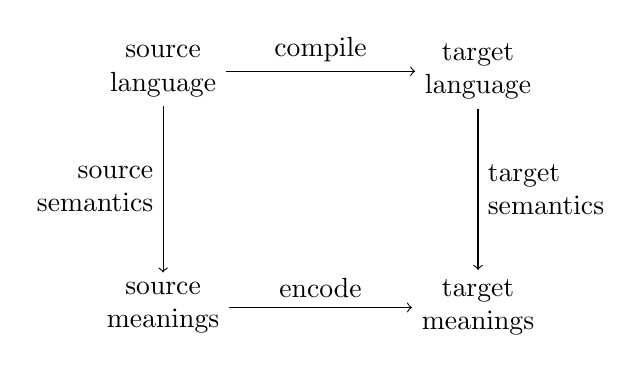
\begin{tikzpicture}
      \node[align=center] (S) at (0cm,3cm) {source\\language};
      \node[align=center] (T) at (4cm,3cm) {target\\language};
      \node[align=center] (M) at (0cm,0cm) {source\\meanings};
      \node[align=center] (U) at (4cm,0cm) {target\\meanings};
      
      \path (S) edge[->] node[align=center, above] {compile}           (T);
      \path (S) edge[->] node[align=right, left]   {source\\semantics} (M);
      \path (T) edge[->] node[align=left, right]   {target\\semantics} (U);
      \path (M) edge[->] node[align=center, above] {encode}            (U);
    \end{tikzpicture}
  \end{center}
  \caption{The commuting diagram used in the traditional approach to compiler verification}
  \label{commuting-diagram}
\end{figure}
Lockwood Morris\cite{morris1973} first observed that the commuting diagram approach was the usual approach to showing compiler correctness, though his version of the diagram had a decode function relating target meanings to source meanings.
Thatcher \emph{et al.}\cite{thatcher1979}, in extending Lockwood Morris' verification of a compiler, noticed that an encode function was more useful in reasoning and so included it in their diagram instead of the decode function.

The commuting diagram approach can be seen in some of the earliest work on compiler correctness, particularly McCarthy and Painter's paper from 1967\cite{mccarthy1967}.
McCarthy and Painter show the correctness of a compiler for a very simple expression language that targets a simple 4-instruction machine.
The source language consists only of constants, variables and addition to form expressions such as $(x + 3) + (y + z)$, and a function that evaluates these expressions to values under a particular variable binding forns the semantics of the source language.
The target machine consists of an acumulator register and a memory store with four instructions:
\begin{itemize}
  \item LI $\alpha$ --- which loads the immediate value $\alpha$ into the accumulator
  \item LOAD $x$ --- which loads a value from the memory location $x$ into the accumulator
  \item STO $x$ --- which stores the value in the accumulator in memory location $x$
  \item ADD $x$ --- which add the value at memory location $x$ to the value in the accumulator
\end{itemize}
The semantics of this target machine are defined by a function that takes an intial state and a list of instructions and outputs the final state.
McCarthy and Painter then define a compilation function from the source language to the target language.
The correctness of the compiler is defined by providing a function that puts the computed value of an expression into the accumulator of a machine state. 
It is then required that applying the function to the result of evaluating an expression is equivalent under a partial equality relation to the resultant state from compiling and running the expression.
The reason for the use of a partial equality is to ensure that any temporary variables introduced in compilation are ignored when comparing the machine states.
Though the use of partial equality and the equational way in which McCarthy and Painter state their definition of compiler correctness obscures it slightly, this can be seen as following the commuting diagram approach as shown in Figure~\ref{mccarthy1967-diagram}.
\begin{figure}
  \begin{center}
    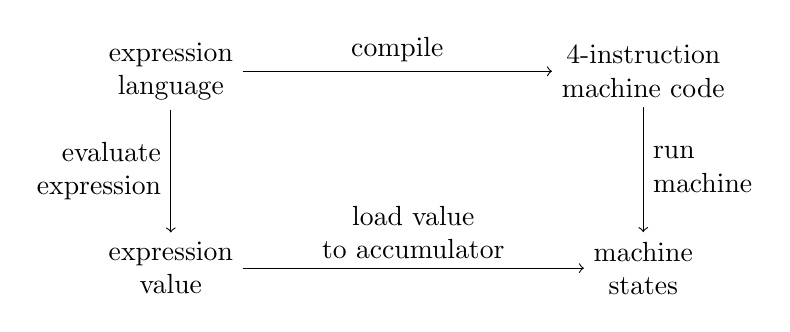
\begin{tikzpicture}
      \node[align=center] (S) at (0cm,2.5cm) {expression\\language};
      \node[align=center] (T) at (6cm,2.5cm) {4-instruction\\machine code};
      \node[align=center] (M) at (0cm,0cm)   {expression\\value};
      \node[align=center] (U) at (6cm,0cm)   {machine\\states};
      
      \path (S) edge[->] node[align=center, above] {compile}                    (T);
      \path (S) edge[->] node[align=right, left]   {evaluate\\expression}       (M);
      \path (T) edge[->] node[align=left, right]   {run\\machine}               (U);
      \path (M) edge[->] node[align=center, above] {load value\\to accumulator} (U);
    \end{tikzpicture}
  \end{center}
  \caption{A diagram showing how McCarthy and Painter's definition of compiler correctness follows the commuting diagram approach}
  \label{mccarthy1967-diagram}
\end{figure}

\section{Research Proposal}

\section{Preliminary Work}

\printbibliography
\end{document}
